\documentclass[conference]{IEEEtran}

% Language setting
% Replace `english' with e.g. `spanish' to change the document language
\usepackage[spanish]{babel}

% Useful packages
\usepackage{amsmath}
\usepackage{graphicx}
\usepackage{url}

% Title and author info
\title{GUITAR HERO, PROTOTIPO 1}
\author{
\IEEEauthorblockN{Ángel Thomas Rodríguez Pinto - 506221014\\ angelt.rodriguezp@konradlorenz.edu.co}
\and
\IEEEauthorblockN{Eddy Andrés Díaz Santos - 506221024\\ eddya.diazs@konradlorenz.edu.co}
}


\begin{document}
\maketitle

\begin{abstract}

The project "GUITAR HERO, PROTOTIPO 1" arises as a result of the practical application of the knowledge in HTML, CSS and JavaScript acquired in class. A prototype inspired by the famous game "Guitar Hero" is developed, with emphasis on an efficient organization of code and multimedia resources. The user interface was designed in a clear and functional way, with keyboard controls for player interaction. The project structure is described in detail, including the division into subfolders and the use of different files for style and functionality. In addition, images showing the final interface of the game are presented. In summary, the project demonstrates a solid mastery of the concepts and skills necessary for web development, evidencing the team's ability to successfully complete complex projects.

\end{abstract}

\section{Introduction}

Se quiso hacer un proyecto en el cual podemos implementar lo visto en clase, como lo son unos de los lenguajes de programacion usados en la historia de la programacion CSS, HTML y JavaScript.
Tras apoyarnos con diferentes herramientas suministradas en clase, se realizo un pequeño prototipo basado en el video juego "Guitar Hero", teniendo en cuenta los diferentes factores que conlleva el videojuego original. 

\section{Creacion}

\subsection{Lenguajes usados}

HTML: Es el lenguaje mas utilizado para crear y diseñar páginas web, la sintaxis de HTML se basa en etiquetas que permiten definir diferentes elementos dentro de una página web, como encabezados, párrafos, imágenes, enlaces, entre otros. Estas etiquetas están rodeadas por corchetes < y >, estos pueden contener atributos para proporcionar información adicional sobre el elemento.
\\
CSS: Este lenguaje tambien esa muy presente en la creacion de paginas web pero centrada al diseño de esta, CSS es muy polivalente ya que permite crear diseños complejos y sofisticados para páginas web. Además, proporciona funcionalidades como la herencia de estilos y la especificidad de selectores, lo que permite un control preciso sobre la apariencia de los elementos de una página web.
\\
JS: Java Script siempre interactua con el contenido HTML y CSS de una página web para proporcionar funcionalidades dinámicas y en tiempo real. Esto incluye acciones como validar formularios, crear animaciones, manipular el DOM (Document Object Model) para cambiar el contenido de una página de manera dinámica y responder a eventos del usuario, como clics de ratón o pulsaciones de teclas.
\subsection{Desarrollo}

Para el desarrollo del prototipo usamos cierta base proporcionada en clase, en la cual hicimos la primera parte que era la inicializacion de movimiento de una figura, ya sea una imagen la cual fue descargada anteriormente o un objeto creado con ayuda del HTML, y el CSS, ya sea un circulo, como en nuestro caso, lo cual representaba las notas del video juego, cada una de estas estaba establecida con un color para poder identificar cada nota, en la interfaz que ve el usuario se quizo especificar como seria el funcionamiento de este y con que teclas se podra jugar. Para esto usamos la clase "main.js", que hace referencia al Java Script donde desde esta clase haremos el funcionamiento de teclas, clics, eliminacion de notas, guardado de puntos, entre otras caracteristicas mas, la clase "Style.css" se realizo todo el diseño de la pagina, como lo son las notas, el contenedor donde van a aparecer las notas, fondos de inicio y de juego, etc. 

\subsection{Division y uso de la interfaz }

La interfaz de usuario que se ve, esta dividida en dos partes primero la pantalla de inicio la cual es la pantalla de carga, que nos da la opcion de iniciar el juego con un boton que contiene el texto de "Iniciar Juego" que al darle clic, este nos lleva inmediantamente a otra pagina donde empieza el juego, y cada que el jugador acierte a una nota se va sumando un punto, mediante que va pasando la cancion, el jugador solamente podra ganar hasta que llegue a la cantidad de 500 notas acertadas. 
Las teclas para poder hacer uso del juego son "A,S,J y K", cada una de estas teclas tiene asignada una nota por ejemplo la letra "A" eliminara las notas de color rojo que esta en su respectiva columna, la letra "S" eliminara las notas de color verde, la letra "J" eliminara las notas de color azul y por ultimo la letra "K" eliminara las notas de color amarillo, asi hasta llegar a los 500 puntos y se detendra el juego. 

\subsection{Division del proyecto }

Para llevar un orden del proyecto se quiso dividir el proyecto en diferentes subcarpetas dentro de una carpeta principal, estas subcarpetas contienen las clases usadas, ya mencionadas anteriormente, son la subcarpeta "css" la cual contiene las dos clases con respecto al estilo del videojuego, "imgs" esta subcarpeta contiene todo el contenido multimedia usado en el juego como lo son sonidos de teclas, musica para una mejor experiencia de usuario, imagenes y videos para fondos y "js" esta ultima subcarpeta contiene la clase que realiza el funcionamiento del juego, en la carpeta principal encontramos dos archivos ".html" estos dos archivos son los que nos permiten abrir el juego, y hacer uso de este. 
\subsection{Imagenes de la interfaz}
Aca podremos ver como la interfaz final que el usuario o jugador podra visualizar a la hora de jugar. 

\centering
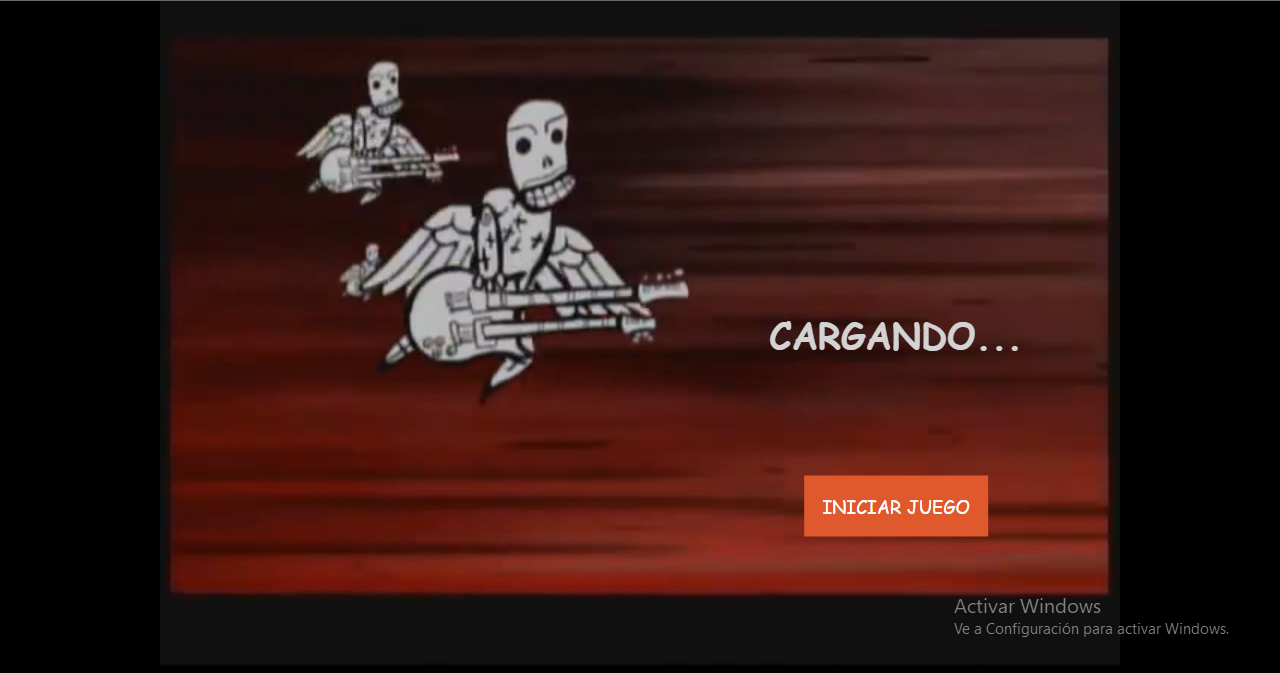
\includegraphics[width=1\linewidth]{Inicio1.png}
Figura 1. Interfaz de inicio antes del juego

\centering
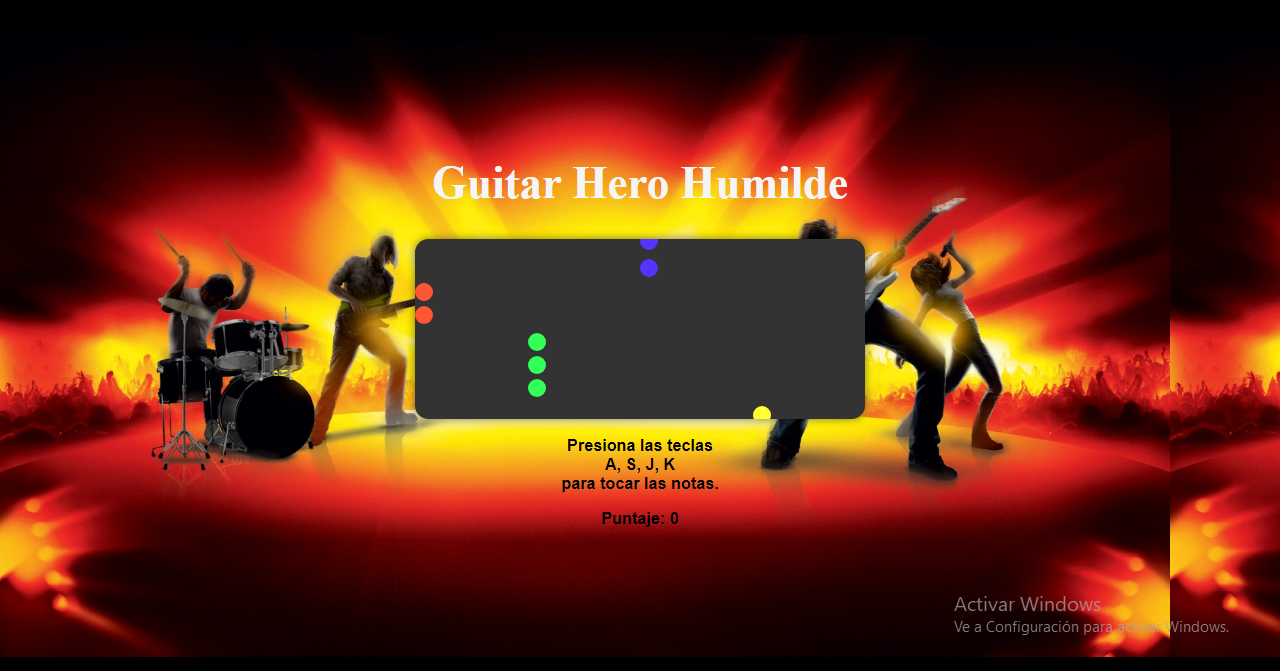
\includegraphics[width=1\linewidth]{Juego1.png}
Figura 2. Interfaz de juego.


\section{Conclusiones}

El proyecto "Guitar Hero, Prototipo 1" destaca por su aplicación efectiva de los conocimientos en HTML, CSS y JavaScript. A través de una organización meticulosa del código y los recursos multimedia, logra una interfaz de usuario clara y funcional. La inclusión de controles de teclado para la interacción con el juego mejora la experiencia del usuario. En conjunto, este prototipo exhibe un sólido entendimiento de los conceptos y habilidades necesarios en el desarrollo web, subrayando la capacidad del equipo para llevar a cabo proyectos de este tipo con éxito.

\bibliography{sample}

\end{document}

